\resizebox{\textwidth}{!}{
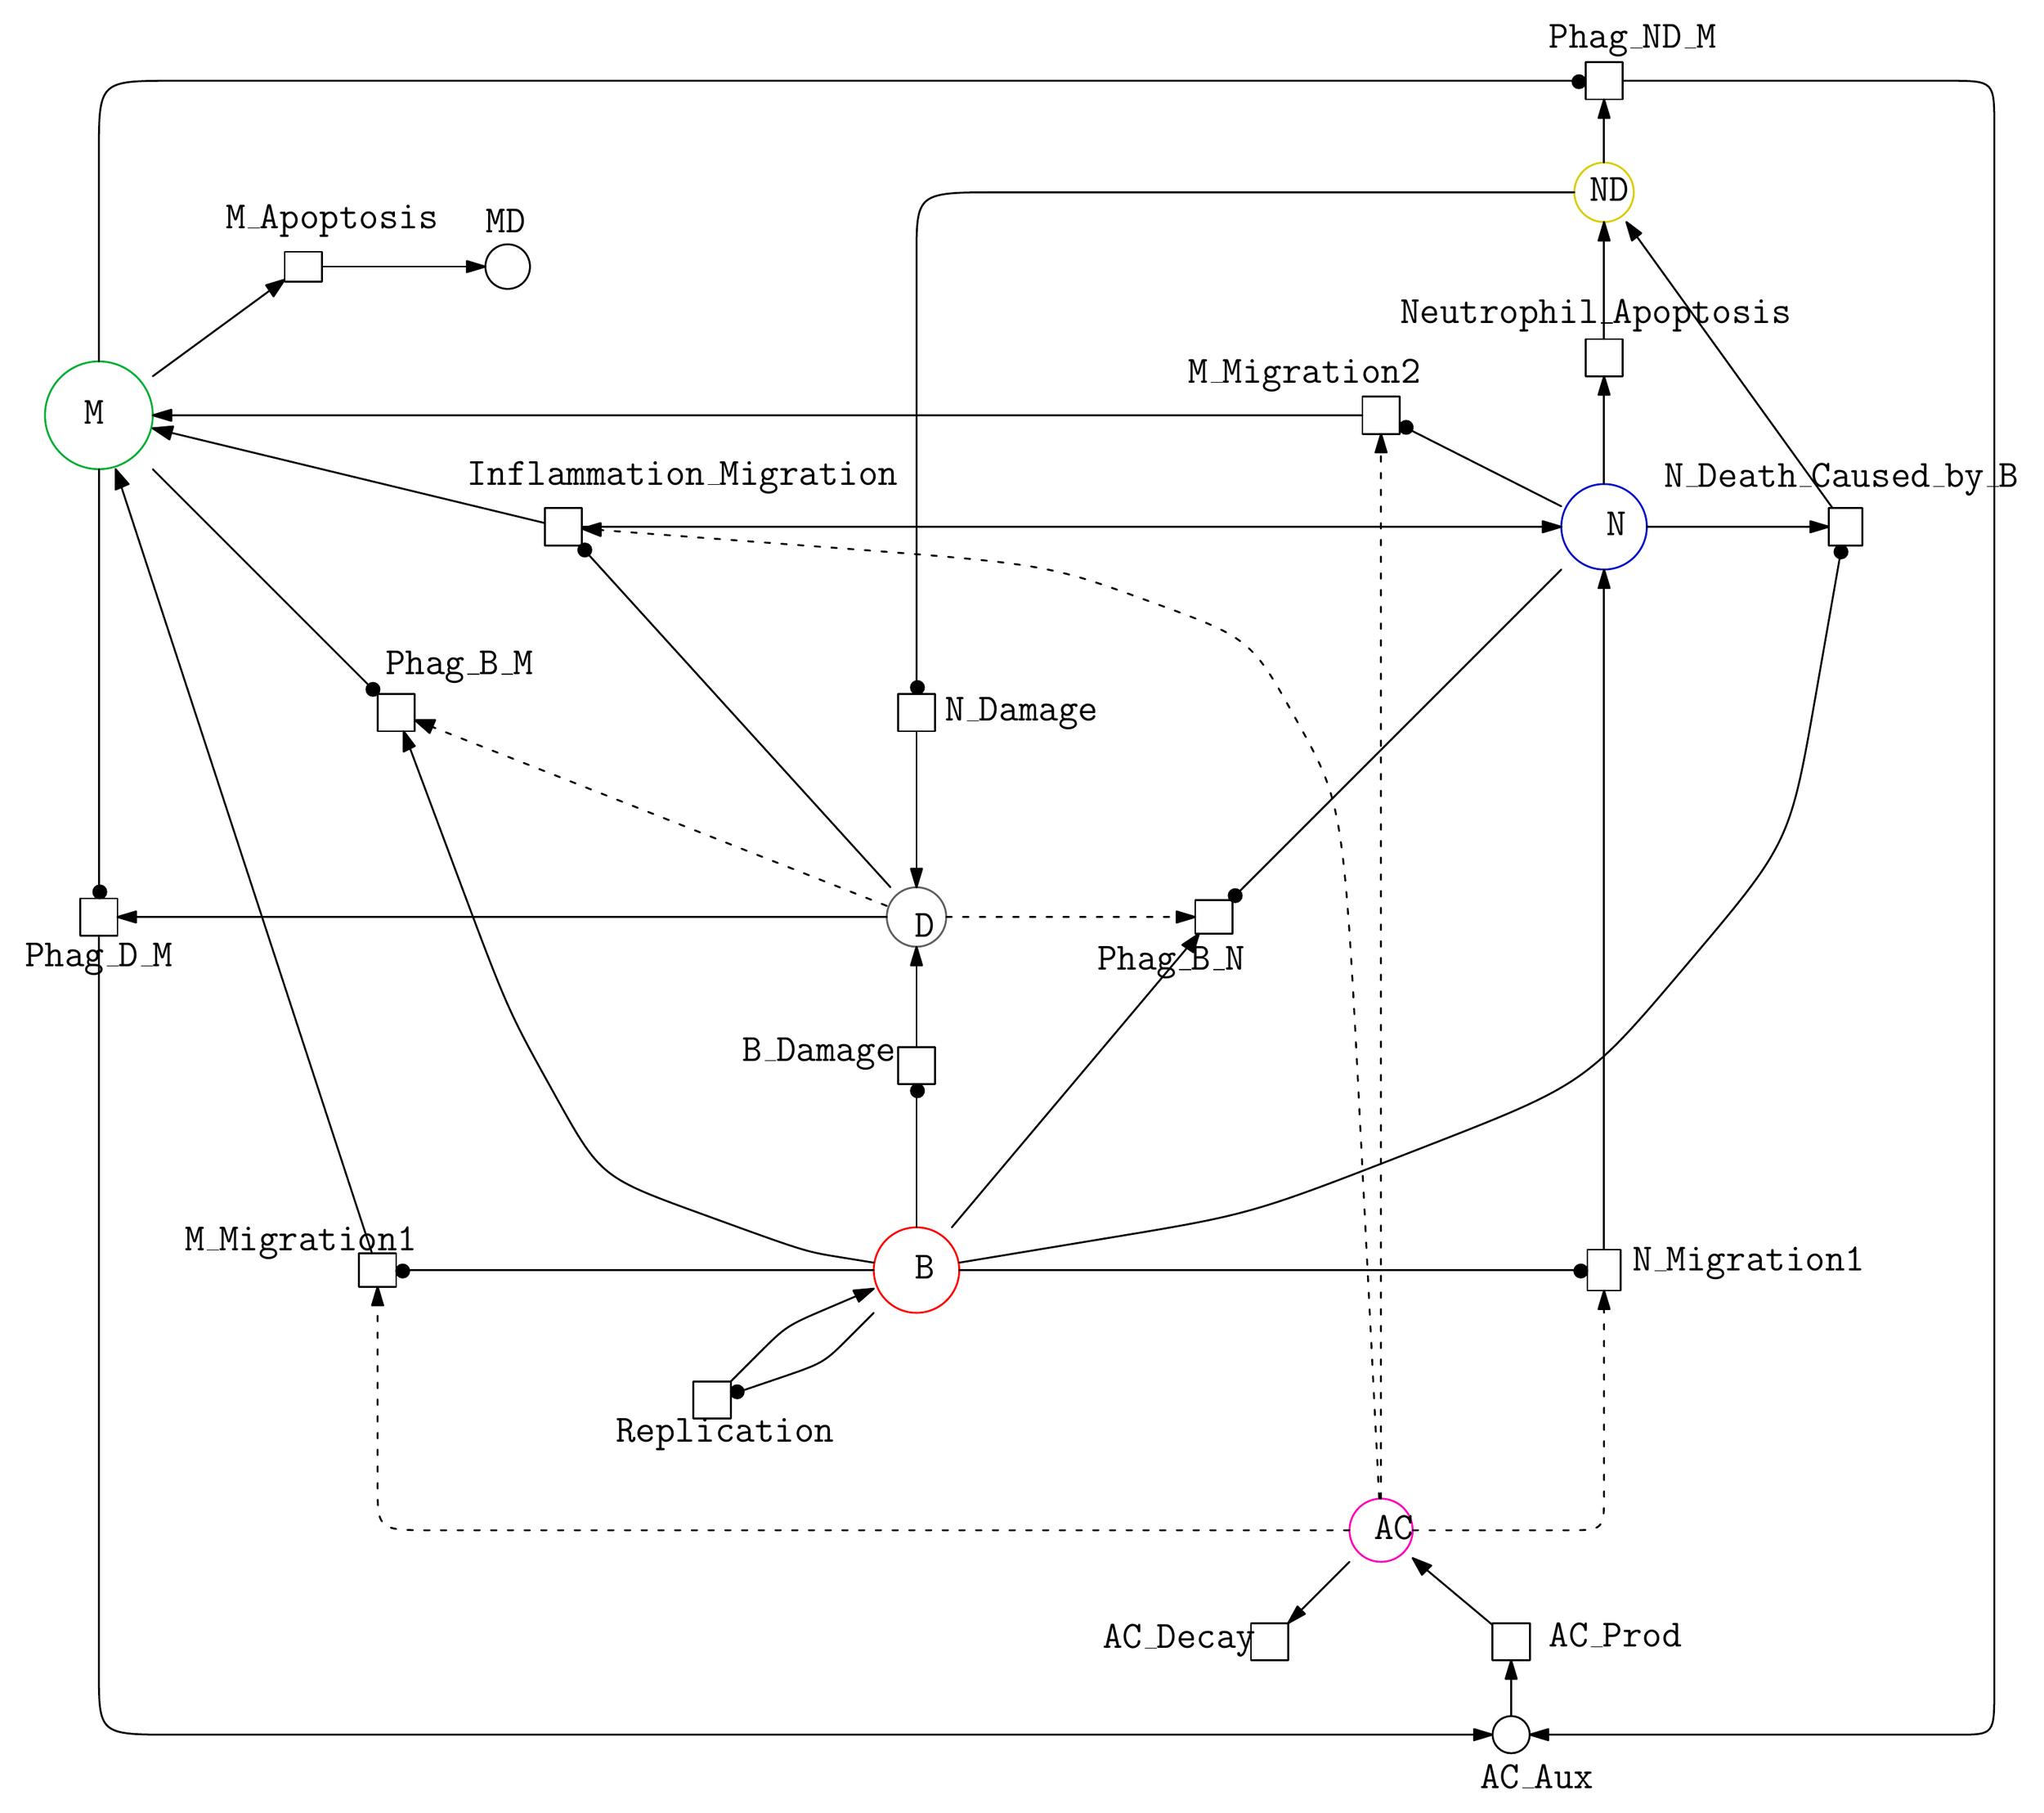
\begin{tikzpicture}[x=1pt,y=-1pt]
\definecolor{r255g3b0}{RGB}{255,3,0}
\definecolor{WHITE}{RGB}{255,255,255}
\draw[r255g3b0, solid, line join=round, line cap=round, line width=1, fill=WHITE]
	(590,870) ellipse[x radius=23, y radius=23];
\definecolor{BLACK}{RGB}{0,0,0}
\draw[BLACK]
	(586,868.5) node[rotate=0, font=\ttfamily\huge, BLACK, right=-.25]
	{B};
\definecolor{r0g16b200}{RGB}{0,16,200}
\draw[r0g16b200, solid, line join=round, line cap=round, line width=1, fill=WHITE]
	(960,470) ellipse[x radius=23, y radius=23];
\draw[BLACK]
	(958,468.5) node[rotate=0, font=\ttfamily\huge, BLACK, right=-.25]
	{N};
\definecolor{r99g94b94}{RGB}{99,94,94}
\draw[r99g94b94, solid, line join=round, line cap=round, line width=1, fill=WHITE]
	(590,680) ellipse[x radius=16, y radius=16];
\draw[BLACK]
	(586,684.5) node[rotate=0, font=\ttfamily\huge, BLACK, right=-.25]
	{D};
\definecolor{r219g204b0}{RGB}{219,204,0}
\draw[r219g204b0, solid, line join=round, line cap=round, line width=1, fill=WHITE]
	(960,290) ellipse[x radius=16, y radius=16];
\draw[BLACK]
	(949,288.5) node[rotate=0, font=\ttfamily\huge, BLACK, right=-.25]
	{ND};
\definecolor{r0g174b51}{RGB}{0,174,51}
\draw[r0g174b51, solid, line join=round, line cap=round, line width=1, fill=WHITE]
	(150,410) ellipse[x radius=29, y radius=29];
\draw[BLACK]
	(139,408.5) node[rotate=0, font=\ttfamily\huge, BLACK, right=-.25]
	{M};
\draw[BLACK, solid, line join=round, line cap=round, line width=1, fill=WHITE]
	(370,330) ellipse[x radius=12, y radius=12];
\draw[BLACK]
	(355,305.5) node[rotate=0, font=\ttfamily\huge, BLACK, right=-.25]
	{MD};
\definecolor{r255g0b183}{RGB}{255,0,183}
\draw[r255g0b183, solid, line join=round, line cap=round, line width=1, fill=WHITE]
	(840,1010) ellipse[x radius=17, y radius=17];
\draw[BLACK]
	(833,1008.5) node[rotate=0, font=\ttfamily\huge, BLACK, right=-.25]
	{AC};
\draw[BLACK, solid, line join=round, line cap=round, line width=1, fill=WHITE]
	(910,1120) ellipse[x radius=10, y radius=10];
\draw[BLACK]
	(890,1142.5) node[rotate=0, font=\ttfamily\huge, BLACK, right=-.25]
	{AC\_Aux};
\draw[BLACK, solid, line join=round, line cap=round, line width=1, fill=WHITE]
	(470,930) rectangle +(20,20);
\draw[BLACK]
	(425,958.5) node[rotate=0, font=\ttfamily\huge, BLACK, right=-.25]
	{Replication};
\draw[BLACK, solid, line join=round, line cap=round, line width=1, fill=WHITE]
	(740,671) rectangle +(20,18);
\draw[BLACK]
	(684,704.5) node[rotate=0, font=\ttfamily\huge, BLACK, right=-.25]
	{Phag\_B\_N};
\draw[BLACK, solid, line join=round, line cap=round, line width=1, fill=WHITE]
	(1081,460) rectangle +(18,20);
\draw[BLACK]
	(989,444.5) node[rotate=0, font=\ttfamily\huge, BLACK, right=-.25]
	{N\_Death\_Caused\_by\_B};
\draw[BLACK, solid, line join=round, line cap=round, line width=1, fill=WHITE]
	(580,560) rectangle +(20,20);
\draw[BLACK]
	(602,570.5) node[rotate=0, font=\ttfamily\huge, BLACK, right=-.25]
	{N\_Damage};
\draw[BLACK, solid, line join=round, line cap=round, line width=1, fill=WHITE]
	(580,750) rectangle +(20,20);
\draw[BLACK]
	(493,753.5) node[rotate=0, font=\ttfamily\bfseries\huge, BLACK, right=-.25]
	{B\_Damage};
\draw[BLACK, solid, line join=round, line cap=round, line width=1, fill=WHITE]
	(140,670) rectangle +(20,20);
\draw[BLACK]
	(107,702.5) node[rotate=0, font=\ttfamily\huge, BLACK, right=-.25]
	{Phag\_D\_M};
\draw[BLACK, solid, line join=round, line cap=round, line width=1, fill=WHITE]
	(300,560) rectangle +(20,20);
\draw[BLACK]
	(301,545.5) node[rotate=0, font=\ttfamily\huge, BLACK, right=-.25]
	{Phag\_B\_M};
\draw[BLACK, solid, line join=round, line cap=round, line width=1, fill=WHITE]
	(950,369) rectangle +(20,20);
\draw[BLACK]
	(847,356.5) node[rotate=0, font=\ttfamily\huge, BLACK, right=-.25]
	{Neutrophil\_Apoptosis};
\draw[BLACK, solid, line join=round, line cap=round, line width=1, fill=WHITE]
	(250,322) rectangle +(20,16);
\draw[BLACK]
	(215,305.5) node[rotate=0, font=\ttfamily\huge, BLACK, right=-.25]
	{M\_Apoptosis};
\draw[BLACK, solid, line join=round, line cap=round, line width=1, fill=WHITE]
	(951,859) rectangle +(18,22);
\draw[BLACK]
	(972,866.5) node[rotate=0, font=\ttfamily\huge, BLACK, right=-.25]
	{N\_Migration1};
\draw[BLACK, solid, line join=round, line cap=round, line width=1, fill=WHITE]
	(290,861) rectangle +(20,18);
\draw[BLACK]
	(193,855.5) node[rotate=0, font=\ttfamily\huge, BLACK, right=-.25]
	{M\_Migration1};
\draw[BLACK, solid, line join=round, line cap=round, line width=1, fill=WHITE]
	(950,220) rectangle +(20,20);
\draw[BLACK]
	(927,208.5) node[rotate=0, font=\ttfamily\huge, BLACK, right=-.25]
	{Phag\_ND\_M};
\draw[BLACK, solid, line join=round, line cap=round, line width=1, fill=WHITE]
	(770,1060) rectangle +(20,20);
\draw[BLACK]
	(687,1069.5) node[rotate=0, font=\ttfamily\huge, BLACK, right=-.25]
	{AC\_Decay};
\draw[BLACK, solid, line join=round, line cap=round, line width=1, fill=WHITE]
	(830,400) rectangle +(20,20);
\draw[BLACK]
	(733,388.5) node[rotate=0, font=\ttfamily\huge, BLACK, right=-.25]
	{M\_Migration2};
\draw[BLACK, solid, line join=round, line cap=round, line width=1, fill=WHITE]
	(390,460) rectangle +(20,20);
\draw[BLACK]
	(345,443.5) node[rotate=0, font=\ttfamily\huge, BLACK, right=-.25]
	{Inflammation\_Migration};
\draw[BLACK, solid, line join=round, line cap=round, line width=1, fill=WHITE]
	(900,1060) rectangle +(20,20);
\draw[BLACK]
	(927,1066.5) node[rotate=0, font=\ttfamily\huge, BLACK, right=-.25]
	{AC\_Prod};
\draw[BLACK, solid, line join=round, line cap=round, line width=1]
	(490,930) -- (505,915) .. controls (520,900) .. (543.5,890) -- (567,880);
\draw[BLACK, solid, line join=round, line cap=round, line width=1, fill=BLACK]
	(567,880) -- (559,887) -- (556,881) -- (567,880) -- cycle;
\draw[BLACK, solid, line join=round, line cap=round, line width=1]
	(609,847) -- (742,689);
\draw[BLACK, solid, line join=round, line cap=round, line width=1, fill=BLACK]
	(742,689) -- (739,699) -- (733,695) -- (742,689) -- cycle;
\draw[BLACK, solid, line join=round, line cap=round, line width=1]
	(983,470) -- (1081,470);
\draw[BLACK, solid, line join=round, line cap=round, line width=1, fill=BLACK]
	(1081,470) -- (1071,473) -- (1071,467) -- (1081,470) -- cycle;
\draw[BLACK, solid, line join=round, line cap=round, line width=1]
	(1083,460) -- (972,306);
\draw[BLACK, solid, line join=round, line cap=round, line width=1, fill=BLACK]
	(972,306) -- (980,312) -- (975,316) -- (972,306) -- cycle;
\draw[BLACK, solid, line join=round, line cap=round, line width=1]
	(590,580) -- (590,664);
\draw[BLACK, solid, line join=round, line cap=round, line width=1, fill=BLACK]
	(590,664) -- (587,654) -- (593,654) -- (590,664) -- cycle;
\draw[BLACK, solid, line join=round, line cap=round, line width=1]
	(590,750) -- (590,696);
\draw[BLACK, solid, line join=round, line cap=round, line width=1, fill=BLACK]
	(590,696) -- (593,706) -- (587,706) -- (590,696) -- cycle;
\draw[BLACK, solid, line join=round, line cap=round, line width=1]
	(574,680) -- (160,680);
\draw[BLACK, solid, line join=round, line cap=round, line width=1, fill=BLACK]
	(160,680) -- (170,677) -- (170,683) -- (160,680) -- cycle;
\draw[BLACK, solid, line join=round, line cap=round, line width=1]
	(567,866) -- (548.5,863) .. controls (530,860) .. (475,840) .. controls (420,820) .. (395,775) .. controls (370,730) .. (342,655) -- (314,580);
\draw[BLACK, solid, line join=round, line cap=round, line width=1, fill=BLACK]
	(314,580) -- (320,588) -- (314,591) -- (314,580) -- cycle;
\draw[BLACK, solid, line join=round, line cap=round, line width=1]
	(960,447) -- (960,389);
\draw[BLACK, solid, line join=round, line cap=round, line width=1, fill=BLACK]
	(960,389) -- (963,399) -- (957,399) -- (960,389) -- cycle;
\draw[BLACK, solid, line join=round, line cap=round, line width=1]
	(960,369) -- (960,306);
\draw[BLACK, solid, line join=round, line cap=round, line width=1, fill=BLACK]
	(960,306) -- (963,316) -- (957,316) -- (960,306) -- cycle;
\draw[BLACK, solid, line join=round, line cap=round, line width=1]
	(179,389) -- (250,337);
\draw[BLACK, solid, line join=round, line cap=round, line width=1, fill=BLACK]
	(250,337) -- (244,346) -- (240,340) -- (250,337) -- cycle;
\draw[BLACK, solid, line join=round, line cap=round, line width=1]
	(270,330) -- (358,330);
\draw[BLACK, solid, line join=round, line cap=round, line width=1, fill=BLACK]
	(358,330) -- (348,333) -- (348,327) -- (358,330) -- cycle;
\draw[BLACK, solid, line join=round, line cap=round, line width=1]
	(960,859) -- (960,493);
\draw[BLACK, solid, line join=round, line cap=round, line width=1, fill=BLACK]
	(960,493) -- (963,503) -- (957,503) -- (960,493) -- cycle;
\draw[BLACK, solid, line join=round, line cap=round, line width=1]
	(297,861) -- (159,439);
\draw[BLACK, solid, line join=round, line cap=round, line width=1, fill=BLACK]
	(159,439) -- (166,447) -- (159,450) -- (159,439) -- cycle;
\draw[BLACK, solid, line join=round, line cap=round, line width=1]
	(960,274) -- (960,240);
\draw[BLACK, solid, line join=round, line cap=round, line width=1, fill=BLACK]
	(960,240) -- (963,250) -- (957,250) -- (960,240) -- cycle;
\draw[BLACK, solid, line join=round, line cap=round, line width=1]
	(823,1027) -- (790,1060);
\draw[BLACK, solid, line join=round, line cap=round, line width=1, fill=BLACK]
	(790,1060) -- (795,1051) -- (799,1055) -- (790,1060) -- cycle;
\draw[BLACK, solid, line join=round, line cap=round, line width=1]
	(830,410) -- (179,410);
\draw[BLACK, solid, line join=round, line cap=round, line width=1, fill=BLACK]
	(179,410) -- (189,407) -- (189,413) -- (179,410) -- cycle;
\draw[BLACK, solid, line join=round, line cap=round, line width=1]
	(410,470) -- (937,470);
\draw[BLACK, solid, line join=round, line cap=round, line width=1, fill=BLACK]
	(937,470) -- (927,473) -- (927,467) -- (937,470) -- cycle;
\draw[BLACK, solid, line join=round, line cap=round, line width=1]
	(390,468) -- (179,417);
\draw[BLACK, solid, line join=round, line cap=round, line width=1, fill=BLACK]
	(179,417) -- (190,416) -- (188,423) -- (179,417) -- cycle;
\draw[BLACK, solid, line join=round, line cap=round, line width=1]
	(900,1061) -- (857,1025);
\draw[BLACK, solid, line join=round, line cap=round, line width=1, fill=BLACK]
	(857,1025) -- (867,1029) -- (862,1034) -- (857,1025) -- cycle;
\draw[BLACK, solid, line join=round, line cap=round, line width=1]
	(910,1110) -- (910,1080);
\draw[BLACK, solid, line join=round, line cap=round, line width=1, fill=BLACK]
	(910,1080) -- (913,1090) -- (907,1090) -- (910,1080) -- cycle;
\draw[BLACK, solid, line join=round, line cap=round, line width=1]
	(150,690) -- (150,870) .. controls (150,1050) .. (150,1085) .. controls (150,1120) .. (190,1120) .. controls (230,1120) .. (565,1120) -- (900,1120);
\draw[BLACK, solid, line join=round, line cap=round, line width=1, fill=BLACK]
	(900,1120) -- (890,1123) -- (890,1117) -- (900,1120) -- cycle;
\draw[BLACK, solid, line join=round, line cap=round, line width=1]
	(970,230) -- (1045,230) .. controls (1120,230) .. (1145,230) .. controls (1170,230) .. (1170,255) .. controls (1170,280) .. (1170,675) .. controls (1170,1070) .. (1170,1095) .. controls (1170,1120) .. (1150,1120) .. controls (1130,1120) .. (1025,1120) -- (920,1120);
\draw[BLACK, solid, line join=round, line cap=round, line width=1, fill=BLACK]
	(920,1120) -- (930,1117) -- (930,1123) -- (920,1120) -- cycle;
\draw[BLACK, solid, line join=round, line cap=round, line width=1]
	(567,893) -- (553.5,906.5) .. controls (540,920) .. (515,928.5) -- (490,937);
\draw[BLACK, solid, line join=round, line cap=round, line width=1, fill=BLACK]
	(493.5,935.5) ellipse[x radius=3.5, y radius=3.5];
\draw[BLACK, solid, line join=round, line cap=round, line width=1]
	(937,493) -- (759,671);
\draw[BLACK, solid, line join=round, line cap=round, line width=1, fill=BLACK]
	(761.5,668.5) ellipse[x radius=3.5, y radius=3.5];
\draw[BLACK, solid, line join=round, line cap=round, line width=1]
	(613,866) -- (691.5,853) .. controls (770,840) .. (860,805) .. controls (950,770) .. (1005,705) .. controls (1060,640) .. (1074,560) -- (1088,480);
\draw[BLACK, solid, line join=round, line cap=round, line width=1, fill=BLACK]
	(1087.5,483.5) ellipse[x radius=3.5, y radius=3.5];
\draw[BLACK, solid, line join=round, line cap=round, line width=1]
	(590,847) -- (590,770);
\draw[BLACK, solid, line join=round, line cap=round, line width=1, fill=BLACK]
	(590.5,773.5) ellipse[x radius=3.5, y radius=3.5];
\draw[BLACK, solid, line join=round, line cap=round, line width=1]
	(150,439) -- (150,670);
\draw[BLACK, solid, line join=round, line cap=round, line width=1, fill=BLACK]
	(150.5,666.5) ellipse[x radius=3.5, y radius=3.5];
\draw[BLACK, solid, line join=round, line cap=round, line width=1]
	(179,439) -- (300,560);
\draw[BLACK, solid, line join=round, line cap=round, line width=1, fill=BLACK]
	(297.5,557.5) ellipse[x radius=3.5, y radius=3.5];
\draw[BLACK, solid, line join=round, line cap=round, line width=1]
	(613,870) -- (951,870);
\draw[BLACK, solid, line join=round, line cap=round, line width=1, fill=BLACK]
	(947.5,870.5) ellipse[x radius=3.5, y radius=3.5];
\draw[BLACK, solid, line join=round, line cap=round, line width=1]
	(567,870) -- (458.5,870) .. controls (350,870) .. (330,870) -- (310,870);
\draw[BLACK, solid, line join=round, line cap=round, line width=1, fill=BLACK]
	(313.5,870.5) ellipse[x radius=3.5, y radius=3.5];
\draw[BLACK, solid, line join=round, line cap=round, line width=1]
	(944,290) -- (812,290) .. controls (680,290) .. (635,290) .. controls (590,290) .. (590,325) .. controls (590,360) .. (590,460) -- (590,560);
\draw[BLACK, solid, line join=round, line cap=round, line width=1, fill=BLACK]
	(590.5,556.5) ellipse[x radius=3.5, y radius=3.5];
\draw[BLACK, solid, line join=round, line cap=round, line width=1]
	(150,381) -- (150,345.5) .. controls (150,310) .. (150,270) .. controls (150,230) .. (190,230) .. controls (230,230) .. (590,230) -- (950,230);
\draw[BLACK, solid, line join=round, line cap=round, line width=1, fill=BLACK]
	(946.5,230.5) ellipse[x radius=3.5, y radius=3.5];
\draw[BLACK, solid, line join=round, line cap=round, line width=1]
	(937,459) -- (850,415);
\draw[BLACK, solid, line join=round, line cap=round, line width=1, fill=BLACK]
	(853.5,416.5) ellipse[x radius=3.5, y radius=3.5];
\draw[BLACK, solid, line join=round, line cap=round, line width=1]
	(576,664) -- (409,480);
\draw[BLACK, solid, line join=round, line cap=round, line width=1, fill=BLACK]
	(411.5,482.5) ellipse[x radius=3.5, y radius=3.5];
\draw[BLACK, loosely dashed, line join=round, line cap=round, line width=1]
	(574,674) -- (320,574);
\draw[BLACK, solid, line join=round, line cap=round, line width=1, fill=BLACK]
	(320,574) -- (331,574) -- (328,581) -- (320,574) -- cycle;
\draw[BLACK, loosely dashed, line join=round, line cap=round, line width=1]
	(857,1010) -- (888.5,1010) .. controls (920,1010) .. (940,1010) .. controls (960,1010) .. (960,990) .. controls (960,970) .. (960,925.5) -- (960,881);
\draw[BLACK, solid, line join=round, line cap=round, line width=1, fill=BLACK]
	(960,881) -- (963,891) -- (957,891) -- (960,881) -- cycle;
\draw[BLACK, loosely dashed, line join=round, line cap=round, line width=1]
	(606,680) -- (740,680);
\draw[BLACK, solid, line join=round, line cap=round, line width=1, fill=BLACK]
	(740,680) -- (730,683) -- (730,677) -- (740,680) -- cycle;
\draw[BLACK, loosely dashed, line join=round, line cap=round, line width=1]
	(840,993) -- (840,420);
\draw[BLACK, solid, line join=round, line cap=round, line width=1, fill=BLACK]
	(840,420) -- (843,430) -- (837,430) -- (840,420) -- cycle;
\draw[BLACK, loosely dashed, line join=round, line cap=round, line width=1]
	(823,1010) -- (591.5,1010) .. controls (360,1010) .. (330,1010) .. controls (300,1010) .. (300,985) .. controls (300,960) .. (300,919.5) -- (300,879);
\draw[BLACK, solid, line join=round, line cap=round, line width=1, fill=BLACK]
	(300,879) -- (303,889) -- (297,889) -- (300,879) -- cycle;
\draw[BLACK, loosely dashed, line join=round, line cap=round, line width=1]
	(839,993) -- (829.5,806.5) .. controls (820,620) .. (795,575) .. controls (770,530) .. (715,510) .. controls (660,490) .. (535,480.5) -- (410,471);
\draw[BLACK, solid, line join=round, line cap=round, line width=1, fill=BLACK]
	(410,471) -- (420,468) -- (420,475) -- (410,471) -- cycle;
\end{tikzpicture}
}

